\chapter{Compiler}
Programmiersprachen dienen als Verständigungsmittel zwischen Programmierern und Rechenanlagen. Diese Sprachen haben sich in der Vergangenheit dabei immer mehr an die  Terminologie eines bestimmtes Anwendungsgebietes angenähert. Durch diese Entwicklung eigneten sich Programmiersprachen direkt für die Dokumentation von entwickelten Algorithmen und Anwendungen, entfernten sich jedoch weiter von den Gegebenheiten des realen Rechners.\footcite[Vgl.][S. 15]{Schneider1975}
\begin{figure}[h]
 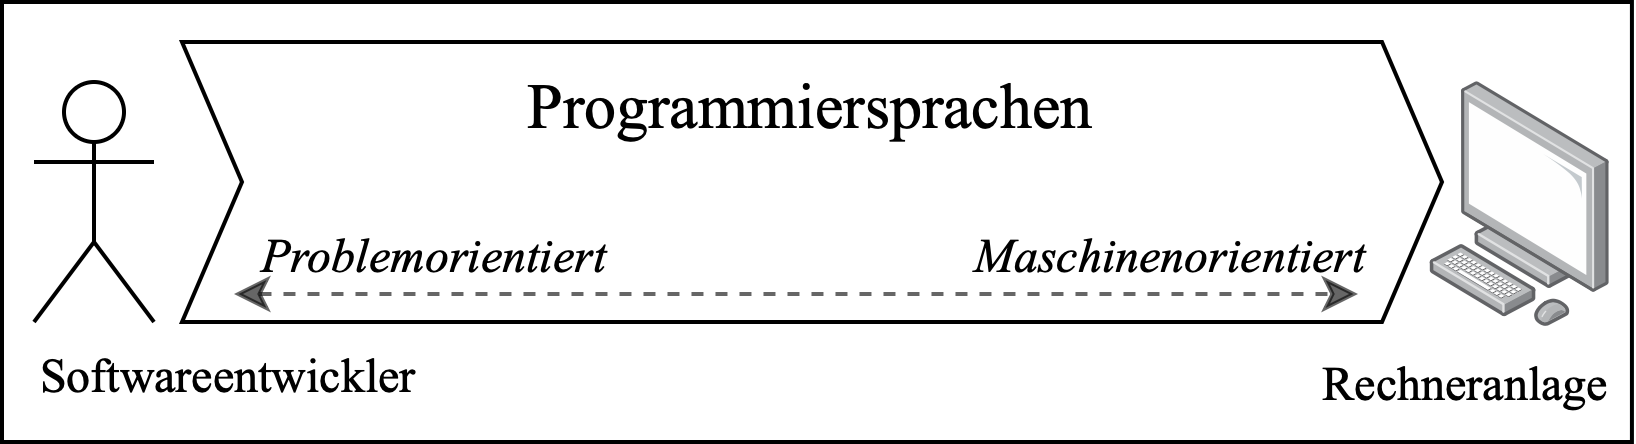
\includegraphics[width=\textwidth,height=\textheight,keepaspectratio]{Images/LanguageIntermediary.png}
 \caption{Programmiersprachen als Schnittstelle}
 \label{fig:Programmiersprachen als Schnittstelle}
\end{figure}
Für die Ausführung einer in einer problemorientierten Programmiersprache geschriebenen Anwendung ist es notwendig, die Sprache in eine maschinenorientierte Form zu überführen. \footcite[Vgl.][S. 15]{Schneider1975} Bereits im Jahre 1952 stelle Rutishauser fest,  dass Computer in der Lage sind diesen Übersetzungsvorgang selbst durchzuführen.\footcite[Vgl.][S. 312]{Rutishauser1952} 
Durch die Möglichkeit zur automatischen Übersetzung von problemorientierten Programmiersprachen konnten Hochsprachen entwickelt werden, die menschenfreundliche Sprachelemente anstatt Maschineninstruktionen verwenden. \footcite[Vgl.][S. 47]{Wagenknecht2014}
\section{ Grundbegriffe}
Diese historische Einführung zeigt,  dass Software zur automatisierten Übersetzung schon seit der Mitte des letzten Jahrhunderts thematisiert wurde, so hat sich in der Wissenschaft eine einheitliche Definition ergeben.  \citeauthor{Ullmann2008} beschreibt die sogenannten Compiler im Jahre \citeyear{Ullmann2008} wie folgt:\footcite[Vgl.][S. 1]{Ullmann2008} 
\begin{Def}[Compiler]
Ein Compiler ist ein Programm, welches ein anderes Programm aus einer Quellsprache in ein gleichwertiges Programm einer Zielsprache übersetzen kann.
\end{Def} 
\vspace{-1em}

Aus dieser Definition lässt sich ein für diese Arbeit relevanter Fakt ableiten: Compiler sind nicht ausschließlich Übersetzer zwischen zwischen problemorientierten,- und maschinenorientierten Programmiersprachen.  Sie sind ausschließlich für die Übersetzung von einer Quellsprache in eine Zielsprache verantwortlich.  Auch wenn der Begriff Programm für jedermann geläufig ist,  kann es dennoch passieren,  das von verschiedenen Repräsentationen eines Programmes gesprochen wird.  So können alle drei der folgenden Begriffe als Programm bezeichnet werden: Der Quelltext, dass ausführbare Programm kann er dennoch unterschiedliche Repräsentationen eines Programmes meinen.  Für das weitere Verständnis dieser Arbeit ist,  mit dem Begriff Programm die ausführbare Anwendung auf den Smartphones des Anwenders gemeint.  

Neben der Übersetzung von problem zu maschinenorientierter Sprache gibt es ebenfalls Compiler, die andere Ziele verfolgen. Dazu gehört zum Beispiel die sogenannten Binärübersetzer,  die den Binärcode eines Programmes für andere Rechner übersetzen, sodass er auf diesen ausgeführt werden kann.  \footcite[Vgl.][S. 27]{Ullmann2008} Ein Source-to-Source(S2S) Compiler,  häufig auch als "Transpiler" bezeichnet,  ist ebenfalls eine besondere Ausprägung eines Compilers die sich wie folgt definieren lässt.  \footcite[Vgl.][S. 1629]{IJCSIT2015}
\begin{Def}[Source-to-Source Compiler]
Ein Source-to-Source-Compiler ist ein Compiler, bei dem sowohl die Quellsprache als auch die Zielsprache eine Hochsprache ist.
\end{Def}
\vspace{-1em}

Der Begriff Hochsprache ist dabei ein Synonym für die bereits eingeführten problemnahen Sprachen wie zum Beispiel C++,  Java,  C\# oder Dart und damit für den Menschen in einer lesbaren und änderbaren Form geschrieben sind. \footcite[Vgl.][S. 9]{Eisenecker2008} 

\section{Compiler Struktur}
Compiler bearbeiten zwei Teilaufgaben für die Übersetzung von Programmen, die Analyse und die Synthese. \footcite[Vgl.][S. 6]{Ullmann2008}\\
Bei der Analyse wird das Programm in seine Bestandteile zerlegt und mit einer grammatischen Struktur versehen. Diese wird anschließend verwendet um eine Zwischendarstellung des Quellprogramms zu erstellen. Dabei wird überprüft, ob das Programm syntaktisch oder semantisch nicht fehlerfrei ist, und ob der Programmierer Änderungen vornehmen muss.  Außerdem werden bei der Analyse Informationen über das Quellprogramm gesammelt und in einer so genannten Symboltabelle abgelegt.  \footcite[Vgl.][S. 6f]{Ullmann2008}

Bei der Synthese wird aus der Zwischendarstellung und den Informationen aus der Symboltabelle das gewünschte Zielprogramm konstruiert. Der Teil des Compilers, der sich mit der Analyse befasst wird oft als Front-End bezeichnet, derjenige der für die Synthese zuständig ist als Back-End.  \footcite[Vgl.][S. 7]{Ullmann2008}

\section{Phasen}
Der Vorgang des Kompilieren lässt sich basierend auf diesen zwei Teilaufgaben nach \citeauthor{Ullmann2008} in mehrere Phasen unterteilen die inAbbildung \ref{fig:Compilerphasen} grafisch dargestellt sind und in diesem Abschnitt detailliert beschrieben werden.  \footcite[Vgl.][S. 6]{Ullmann2008}

\begin{figure}[!ht]
 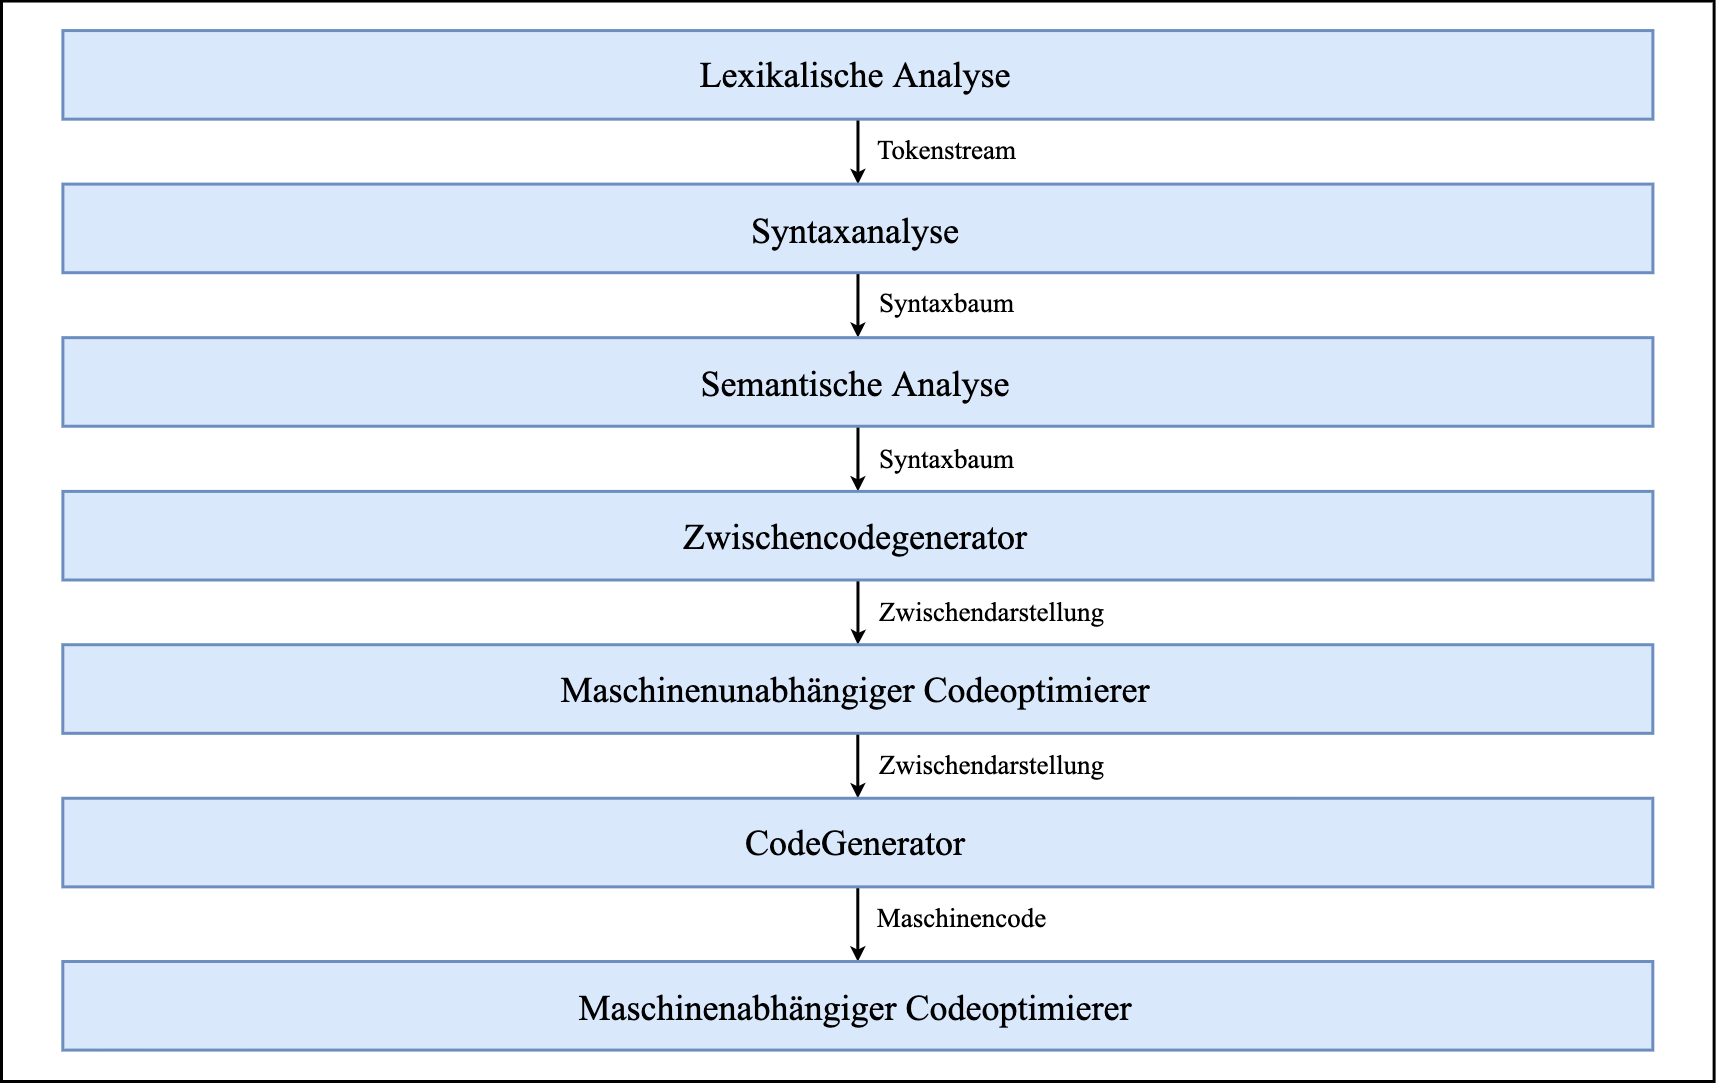
\includegraphics{Images/Compiler/Phasen.png}
 \caption[Phasen eines Compilers]{Phasen eines Compilers\protect\footnotemark}
 \label{fig:Compilerphasen}
\end{figure}
\footnotetext{Abbildung in Anlehnung an Ullman et al. 2008, S.6.}


\subsection{Lexikalische Analyse}
Die erste Phase eines Compilers ist die lexikalische Analyse die sich mit der Untergliederung des Quelltextes in Lexeme beschäftigt.  Ein Lexem ist die Folge von Zeichen im Quellprogramm,  die als Instanz eines Tokens erkannt wurden.  Dabei ist ein Token ein Paar aus Namen und einem optionalen Attributwert wobei der Name zum Beispiel ein bestimmtes Schlüsselwort oder eine Folge von Eingabezeichen seien kann und der Attributwert auf einen Eintrag in der Symboltabelle zeigt.  \footcite[Vgl.][S. 135 f.]{Ullmann2008} In Tabelle \ref{tab:Tokens} werden einige Beispielhafte Tokens aufgeführt und aus welchen Lexemen diese extrahiert werden.

\begin{table}[!ht]
\begin{tabular}{|l|l|l|}
\hline
\textbf{Token} & \textbf{Beschreibung} & \textbf{Beispiellexeme} \\ \hline
if             & Zeichen i,f           & if                      \\ \hline
comparison     & Vergleichsoperatoren  & \textless{}=            \\ \hline
id             & Buchstaben            & pi                      \\ \hline
number         & Numerische Konsten    & 3.14159                 \\ \hline
\end{tabular}

\caption[Token-Beispiele]{Token-Beispiele\protect\footnotemark}
 \label{tab:Tokens}
\end{table}
\footnotetext{Abbildung in Anlehnung an Ullman et al. 2008, S.137}

Basierend auf dieser Beschreibung ist in \ref{fig:LexerResult} ein Beispiel dargestellt, welches zeigt wie der Lexer aus einem Zeichenstring mehrere Token mit den optionalen Attributwerten generiert.  
 
\begin{figure}[!ht]
 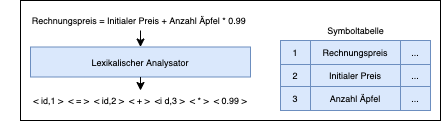
\includegraphics{Images/Compiler/LexerResult.png}
 \caption[Lexer Beispiel]{Lexer Beispiel\protect\footnotemark}
 \label{fig:LexerResult}
\end{figure}
\footnotetext{Abbildung in Anlehnung an Ullman et al. 2008, S.10.}

Der Lexer interagiert mit den anderen Komponenten eines Compilers, diese  Beziehungen werden in Abbildung \ref{fig:LexerInteraktionen}  dargestellt.  Dabei wird der Lexer häufig durch den Parser aufgerufen,  dies wird in der Abbildung mit dem Aufruf "getNextToken" dargestellt.  \footcite[Vgl.][S. 135]{Ullmann2008} 

\begin{figure}[!ht]
 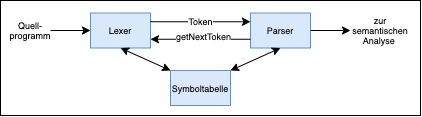
\includegraphics{Images/Compiler/Lexer.png}
 \caption[Interaktion zwischen Lexer und Parser]{Interaktion zwischen Lexer und Parser\protect\footnotemark}
 \label{fig:LexerInteraktionen}
\end{figure}
\footnotetext{Abbildung in Anlehnung an Ullman et al. 2008, S.135.}




Da der Lexer derjenige Teil des Compilers ist, der den Quelltext liest, kann er neben der Identifikation von Lexemen auch weitere Aufgaben übernehmen. So eignet er sich Ideal zum Streichen von Kommentaren im Quelltext und zum entfernen von Leerstellen wie Leerzeichen und Tabulatoren.  Eine weitere essentielle Aufgabe des Lexers ist es eine Zuordnung von Zeilennummern zu gefunden Fehlern herstellen zu können.  Bei einem Fehler wärend der Kompilierung kann somit ein Fehler an den Entwickler ausgegeben werden mit einem genauen Hinweis,  wo der Fehler aufgetreten ist.  \footcite[Vgl.][S. 135.]{Ullmann2008} 
Häufig werden Lexer daher in zwei Kaskadierende Prozesse unterteilt, einem Löschen von Kommentaren und Zusammenfassen von Leerraumzeichen und einen für die eigentliche lexikalische Analyse.  \footcite[Vgl.][S. 136.]{Ullmann2008} 

\subsection{Syntaxanalyse}
Die zweite Phase des Compilers ist die Syntaxanalye.  Dafür verwendet der sogenannte Parser die vom lexikalischen Analysator ausgegebenen Token um eine baumartige Zwischendarstellung zu erstellen, die die grammatische Struktur der Tokens zeigt.  Die Darstellung wird daher auch häufig als Syntaxbaum bezeichnet.  \footcite[Vgl.][S. 9]{Ullmann2008} Abbildung \ref{fig:ParserInteraktionen} zeigt die Position von Pasern in Compilern mitsamt der Übergabe des Syntaxbaums an die nächste Phase. 

\begin{figure}[!ht]
 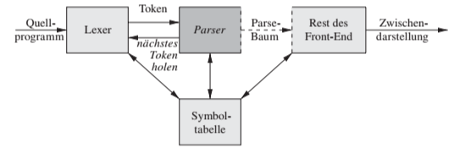
\includegraphics{Images/Compiler/ParserStellung.png}
 \caption[Position von Parsern in Compilern]{Position von Parsern in Compilern\protect\footnotemark}
 \label{fig:ParserInteraktionen}
\end{figure}
\footnotetext{Abbildung in Anlehnung an Ullman et al. 2008, S.233.}

Die Knoten stehen dabei für eine Operation und seine Kindknoten für die Argumente dieser Operation. Die Anordnung der Operationen stimmt mit üblichen arithmentischen Konventionen überein, wie zum Beispiel der vorrang der Multiplikation vor Addition. 


\subsection{Semantische Analyse}
Bei der semantischen Analyse wird der Syntaxbaum und die Informationen aus der Symboltabelle verwendet um das Quellprogramm auf semantische Konsistenz mit der Sprachdefinition zu überprüfen. Außerdem werden in dieser Typinformationen gesammelt und entweder im Syntaxbaum oder in der Symboltabelle hinterlegt um sie in späteren Phasen zu verwenden. Dabei werden außerdem Typen überprüft, daher analysiert ob jeder Operator die passenden Operanden hat. \footcite[Vgl.][S. 9ff]{Ullmann2008}
\subsection{Zwischencodeerzeugung}
Bei der Übersetzung eines Quellprogramms in den Zielcode kann der Compiler mehrere Zwischendarstellungen in verschiedenen Formen erstellen. Syntaxbäume sind beispielsweise eine solche Darstellung. Nach der semantischen Analyse stellen viele Compiler eine maschinennahe Zwischendarstellung die für eine Abstrakte Maschine entworfen wurden.  \footcite[Vgl.][S. 11]{Ullmann2008}
\subsection{Codeoptimierung}
In dieser Phase wird der maschinenunabhängige Code so optimiert, dass sich darauf ein besserer Zielcode ergibt. Dabei bedeutet besser, schnellerer code oder code der weniger Ressourcen verbraucht. Der Umfang der Codeoptimierung schwankt dabei von Compiler zu Compiler erheblich.  \footcite[Vgl.][S. 11f]{Ullmann2008}
\subsection{Codeerzeugung}
Bei der Codeerzegung werden die Eingaben aus der Zwischendarstellung des Quellprogramms entgegengenommen und auf die Zielsprache abgebildet. Ein entsheidender Aspekt der Codeerzeugung ist die sinnvolle zuweisung von Registern für Variablen, falls es sich bei der Zielsprache um Maschinencode handelt.\footcite[Vgl.][S. 13]{Ullmann2008}



Wär

Die Syntax einer Programmiersprache ist das Aussehen bzw. die Struktur des Quelltextes. Der komplette Quelltext eines Programms muss syntaktisch korrekt sein, damit er übersetzt werden kann.  \\
Die Semantik ist die Bedeutung, die den verschiedenen syntaktischen Strukturen zugeordnet werden kann. Es ist also von der Semantik abhängig auf welche Art und Weise die Weiterverabeitung durch den Compiler erfolgt. 


